
%%--------------------------------------------------
%% Holt: Multiple Choice Questions
%%--------------------------------------------------


%% Chapter 04: Forces and the Laws of Motion
%%--------------------------------------------------


%% Holt Multiple Choice Questions
%%--------------------------------------------------
\element{holt-mc}{
\begin{question}{holt-ch04-Q01}
    Two blocks of masses $m_1$ and $m_2$ are placed in contact with each other on a smooth, horizontal surface.
    Block $m_1$ is on the left of block $m_2$.
    A constant horizontal force $F$ to the right is applied to $m_1$
    What is the acceleration of the two blocks?
    \begin{multicols}{2}
    \begin{choices}
        \wrongchoice{$\dfrac{F}{m_1}$}
        \wrongchoice{$\dfrac{F}{m_2}$}
      \correctchoice{$\dfrac{F}{m_1+m_2}$}
        \wrongchoice{$\dfrac{F}{m_1m_2}$}
    \end{choices}
    \end{multicols}
\end{question}
}

\element{holt-mc}{
\begin{question}{holt-ch04-Q02}
    Two blocks of masses $m_1$ and $m_2$ are placed in contact with each other on a smooth, horizontal surface.
    Block $m_1$ is on the left of block $m_2$.
    A constant horizontal force $F$ to the right is applied to $m_1$
    What is the horizontal force acting on $m_2$?
    \begin{multicols}{2}
    \begin{choices}
        %% F_1 = m_1 \frac{F}{m_2+m_2}
      \correctchoice{$\dfrac{F m_1}{m_1+m_2}$}
        \wrongchoice{$\dfrac{F m_2}{m_1+m_2}$}
        %\wrongchoice{$\dfrac{F}{m_2}$}
        \wrongchoice{$\dfrac{F \left(m_1+m_2\right)}{m_2}$}
        \wrongchoice{$\dfrac{F \left(m_1+m_2\right)}{m_1}$}
        %\wrongchoice{$m_1 a$}
        %\wrongchoice{$m_2 a$}
        %\wrongchoice{$(m_1 + m_2) a$}
        %\wrongchoice{$m_1 m_2 a$}
    \end{choices}
    \end{multicols}
\end{question}
}

\element{holt-mc}{
\begin{question}{holt-ch04-Q03}
    A crate is pulled to the right (positive $x$-axis)
        with a force of \SI{82}{\newton},
        to the left with a force of \SI{115}{\newton},
        upward with a force of \SI{565}{\newton},
        and downward with a force of \SI{236}{\newton}.
    Find the magnitude and direction of the net force on the crate.
    \begin{choices}
        \wrongchoice{\SI{3.30}{\newton} at \ang{96} counterclockwise from the positive $x$-axis}
        \wrongchoice{\SI{3.30}{\newton} at \ang{6} counterclockwise from the positive $x$-axis}
      \correctchoice{\SI{3.30e2}{\newton} at \ang{96} counterclockwise from the positive $x$-axis}
        \wrongchoice{\SI{3.30e2}{\newton} at \ang{6} counterclockwise from the positive $x$-axis}
    \end{choices}
\end{question}
}

\element{holt-mc}{
\begin{question}{holt-ch04-Q04}
    A ball with a mass of $m$ is thrown into the air,
        as shown in the figure below.
    \begin{center}
    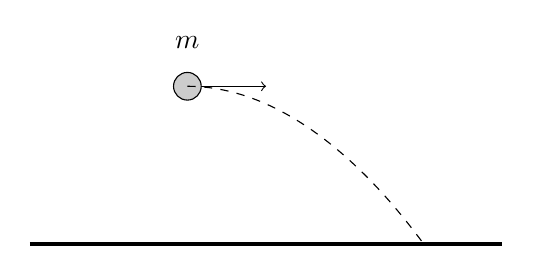
\begin{tikzpicture}
        \draw[->] (0,0) -- ++(0:1);
        \draw[fill=white!80!black] (0,0) circle (0.5em) node[above=1em] {$m$};
        \draw[dashed] (0,0) parabola bend (0,0) (3,-2);
        \draw[ultra thick] (-2,-2) -- (4,-2);
    \end{tikzpicture}
    \end{center}
    What is the force exerted on Earth by the ball?
    \begin{choices}
        \wrongchoice{$m_{ball} g$, directed down}
      \correctchoice{$m_{ball} g$, directed up}
        \wrongchoice{$m_{earth} g$, directed down}
        \wrongchoice{$m_{earth} g$, directed up}
    \end{choices}
\end{question}
}

\element{holt-mc}{
\begin{question}{holt-ch04-Q05}
    A freight train has a mass of \SI{1.5e7}{\kilo\gram}.
    If the locomotive can exert a consant pull of \SI{7.5e5}{\newton},
        how long would it take to increase the speed of the train from rest to \SI{85}{\kilo\meter\per\hour}?
    (Disregard friction)
    \begin{multicols}{2}
    \begin{choices}
      \correctchoice{\SI{4.7e2}{\second}}
        \wrongchoice{\SI{4.7}{\second}}
        \wrongchoice{\SI{5.0e-2}{\second}}
        \wrongchoice{\SI{5.0e4}{\second}}
    \end{choices}
    \end{multicols}
\end{question}
}

\element{holt-mc}{
\begin{question}{holt-ch04-Q06}
    A truck driver slams on the brakes and skids to a stop through a displacement $\Delta x$.
    If the truck's mass doubles,
        find the truck's skidding distance in terms of $\Delta x$:
        (Hint: Increasing the mass increases the normal force)
    \begin{multicols}{2}
    \begin{choices}
        \wrongchoice{$\dfrac{\Delta x}{4}$}
      \correctchoice{$\Delta x$}
        \wrongchoice{$2 \Delta x$}
        \wrongchoice{$4 \Delta x$}
    \end{choices}
    \end{multicols}
\end{question}
}

\element{holt-mc}{
\begin{question}{holt-ch04-Q07}
    A truck driver slams on the brakes and skids to a stop through a displacement $\Delta x$.
    If the truck's initial velocity were halved,
        what would be the truck's skidding distance.
    \begin{multicols}{2}
    \begin{choices}
      \correctchoice{$\dfrac{\Delta x}{4}$}
        \wrongchoice{$\Delta x$}
        \wrongchoice{$2 \Delta x$}
        \wrongchoice{$4 \Delta x$}
    \end{choices}
    \end{multicols}
\end{question}
}

\newcommand{\holtChFourQEight}{
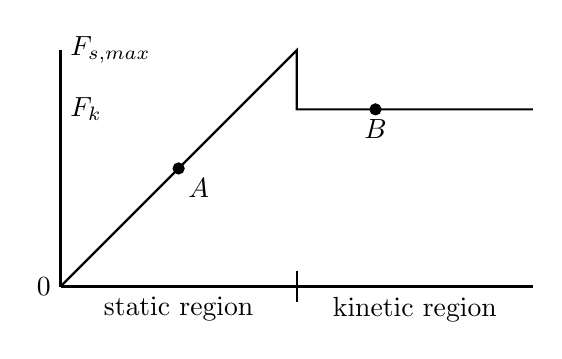
\begin{tikzpicture}
    %% X and Y axis
    \draw[thick] (0,0) -- (6,0);
    \draw[thick] (0,0) -- (0,3);
    %% X and Y axis
    \node[anchor=west] at (0,2.25) {$F_k$};
    \node[anchor=west] at (0,3.00) {$F_{s,max}$};
    \node[anchor=east] at (0,0) {$0$};
    %% X axis regions
    \draw[thick] (0,0) -- (3,0) node [pos=0.5,anchor=north] {static region};
    \draw[thick] (3,0) -- (6,0)  node [pos=0.5,anchor=north] {kinetic region};
    \draw[thick] (3,-0.2) -- (3,0.2);
    %% Graph line
    \draw[thick] (0,0) -- (3,3) -- (3,2.25) -- (6,2.25);
    \draw[fill] (1.5,1.5) circle (2pt) node[anchor=north west] {$A$};
    \draw[fill] (4,2.25) circle (2pt) node[anchor=north] {$B$};
\end{tikzpicture}
}

\element{holt-mc}{
\begin{question}{holt-ch04-Q08}
    The graph below shows the relationship between the applied force ($x$-axis) and the net force of friction ($y$-axis).
    \begin{center}
        \holtChFourQEight
    \end{center}
    What is the relationship between the forces at point $A$?
    \begin{multicols}{2}
    \begin{choices}
      \correctchoice{$F_s = F_{applied}$}
        \wrongchoice{$F_k = F_{applied}$}
        \wrongchoice{$F_s < F_{applied}$}
        \wrongchoice{$F_k > F_{applied}$}
    \end{choices}
    \end{multicols}
\end{question}
}

\element{holt-mc}{
\begin{question}{holt-ch04-Q09}
    The graph below shows the relationship between the applied force ($x$-axis) and the net force of friction ($y$-axis).
    \begin{center}
        \holtChFourQEight
    \end{center}
    What is the relationship between the forces at point $B$?
    \begin{multicols}{2}
    \begin{choices}
        \wrongchoice{$F_{s,max} = F_{k}$}
        \wrongchoice{$F_k > F_{s,max}$}
        \wrongchoice{$F_k > F_{applied}$}
      \correctchoice{$F_k < F_{applied}$}
    \end{choices}
    \end{multicols}
\end{question}
}


\endinput


